% 
% Sample latex source for a project report
%
% This is intended as an introduction to latex, but includes some
% advice about what you might want for the content of your paper
%
% Jim Teresco
% Williams College, Mount Holyoke College, Siena College, The College
% of Saint Rose
%
% Last modified: Mon Dec  4 19:03:24 EST 2017
%
%
% Modified by: Pat Baumgardner, Adam Dachenhausen, Shah Syed
%
%
% First, as you may have guessed, % is the way to define a latex 
% comment
%
% The first line tells latex you want for a default font size and that
% you want to create an ``article''
\documentclass[12pt]{article}
% extra packages to bring in
\usepackage{latexsym}
\usepackage{graphicx}      % extended graphics package
\usepackage{epsfig}        % wrapper for graphicx package
\usepackage{times}
\usepackage{url}
% set some margins, these can be defined as in, cm, pt
\setlength{\topmargin}{-0.5in}
\setlength{\textheight}{9in}
\setlength{\oddsidemargin}{0in}
\setlength{\evensidemargin}{0in}
\setlength{\textwidth}{6.5in}

% a few macros that might be useful -- any time we type \eg it expands
% to the italicized version defined here
\newcommand{\etal}{{\it et al}.$\:$}
\newcommand{\eg}{{\it e}.{\it g}.$\:$}
\newcommand{\cf}{{\it cf}.$\:$}
\newcommand{\ie}{{\it i}.{\it e}.$\:$}

%% to remove page numbers, uncomment this:
%% \pagestyle{empty}

%% Define single-space command
\newcommand{\singlespace}{
  \protect\renewcommand\baselinestretch{1.0}
  \protect\normalsize
}
% use this instead if you want to disable it completely:
%%\newcommand{\singlespace}{}

%% Define double-space command (really more like 1.5 spacing)
%% This is essential for rough drafts, and not a bad idea even for
%%  final submissions
\newcommand{\doublespace}{
  \protect\renewcommand\baselinestretch{1.5}
  \protect\normalsize
}
% use this instead if you want to disable it completely:
%%\newcommand{\doublespace}{}

% This tells latex we're done defining the preamble stuff and we're
% ready to start writing the document
\begin{document}

% this removes the date that is automatically placed in the title.
% comment it out if you want the date
\date{}

% the next few items define things to go onto the title section, like,
% well, the title, and the list of authors
\title{Java Based Memory Latency Simulator}

\author{Pat Baumgardner, Adam Dachenhausen, Shah Syed\\
Department of Computer Science\\
Siena College\\
Loudonville, NY  12211
}

% this tells latex that you're done setting up title stuff and that it
% should go ahead and generate the title here
\maketitle
% leave the page number off but for this page only
\thispagestyle{empty}

% Abstract!
\begin{abstract}
It's usually a good idea to include an abstract.  This should be a
brief summary of your paper.  Highlight your important results.  A
half a page is about right.  Maybe less.  It should be independent of
your subsequent introduction/overview section.
\end{abstract}

% turn on double spacing
\doublespace

% Now we write the text of the paper, hopefully breaking it up into
% nice sections and subsections, using figures and tables as
% appropriate, and referring to those sections using labels instead of
% trying to number things by hand
\section{Overview}
\label{sec:overview}

Begin with an introduction to your topic, specifically emphasizing
what you have done.  Some historical background and references to
related projects are appropriate.  You should also outline the paper
in the overview section.  It might go something like this:

In Section~\ref{sec:vectarray} we discuss how to build a vector from
an array.  Section~\ref{sec:subsections} has a lot of examples of
things you might want \LaTeX~\cite{lamport86} to do.  In
Section~\ref{sec:writing}, we discuss how writing is hard and offer
some suggestions on how to do a better job at it.
Section~\ref{sec:building} describes how to use \LaTeX{} to compile
this document into printable postscript.  Finally,
Section~\ref{sec:conclusions} summarizes the results and presents
suggestions for future work.

Notice how references are used instead of actual section numbers.
This allows you to move, add, or remove sections and have the section
numbers stay correct.  The names are specified below with label commands.

\section{Building a Vector from an Array}
\label{sec:vectarray}

This section is here to give examples of math mode, font changes, the
verbatim environment, and importing a postscript figure.

This experiment measures the time taken to copy an array of $n$ {\tt
int} values to a {\tt Vector} of $n$ {\tt Integer} objects.  We will
use the {\tt add()} method of {\tt class Vector} to append new
values to the end of the vector.  Accessing each item in the array is
a constant time ($O(1)$) operation, as are the construction of the
{\tt Integer} object which will hold the value in the vector and each
{\tt add()} call.  We do this for each of $n$ items, thus, we
expect this operation to take $O(n)$ time.  We create our vector to be
initially of size $n$ to avoid the need to resize dynamically during
the experiments.  We use the {\tt Vector} implementation found in the
{\tt structure} package.


{\it Now, we describe how the experiment is set up, how you run it, and
present and discuss the results.  This sentence is mainly inserted to
show an example of italics.}

A simple Java program was written to copy of an array into the
vector.  A method called {\tt copy()} takes the value of $n$ as its
parameter, creates and fills an array of size $n$, creates an empty
{\tt Vector}, starts a timer, copies the values from the array to the
vector, stops the timer, and prints out the time taken.  The body of
this method is shown in Figure~\ref{fig:code}.

{\singlespace % we don't want to doublespace our code snippet
\begin{figure}[htb]
\begin{verbatim}
    int[] array = new int[n];
    int i;
    for (i=0; i<n; i++) array[i]=i;
	
    Vector v = new Vector(n);
    long start=System.currentTimeMillis();
    for (i=0; i<n; i++) {
        v.add(new Integer(array[i]));
    }
    long end = System.currentTimeMillis();
    System.out.println("For n="+n+", time="+(end-start));
\end{verbatim}
\caption{Java source to copy an array to a Vector.}
\label{fig:code}
\end{figure}
}

\begin{figure}[htb]
\begin{center}
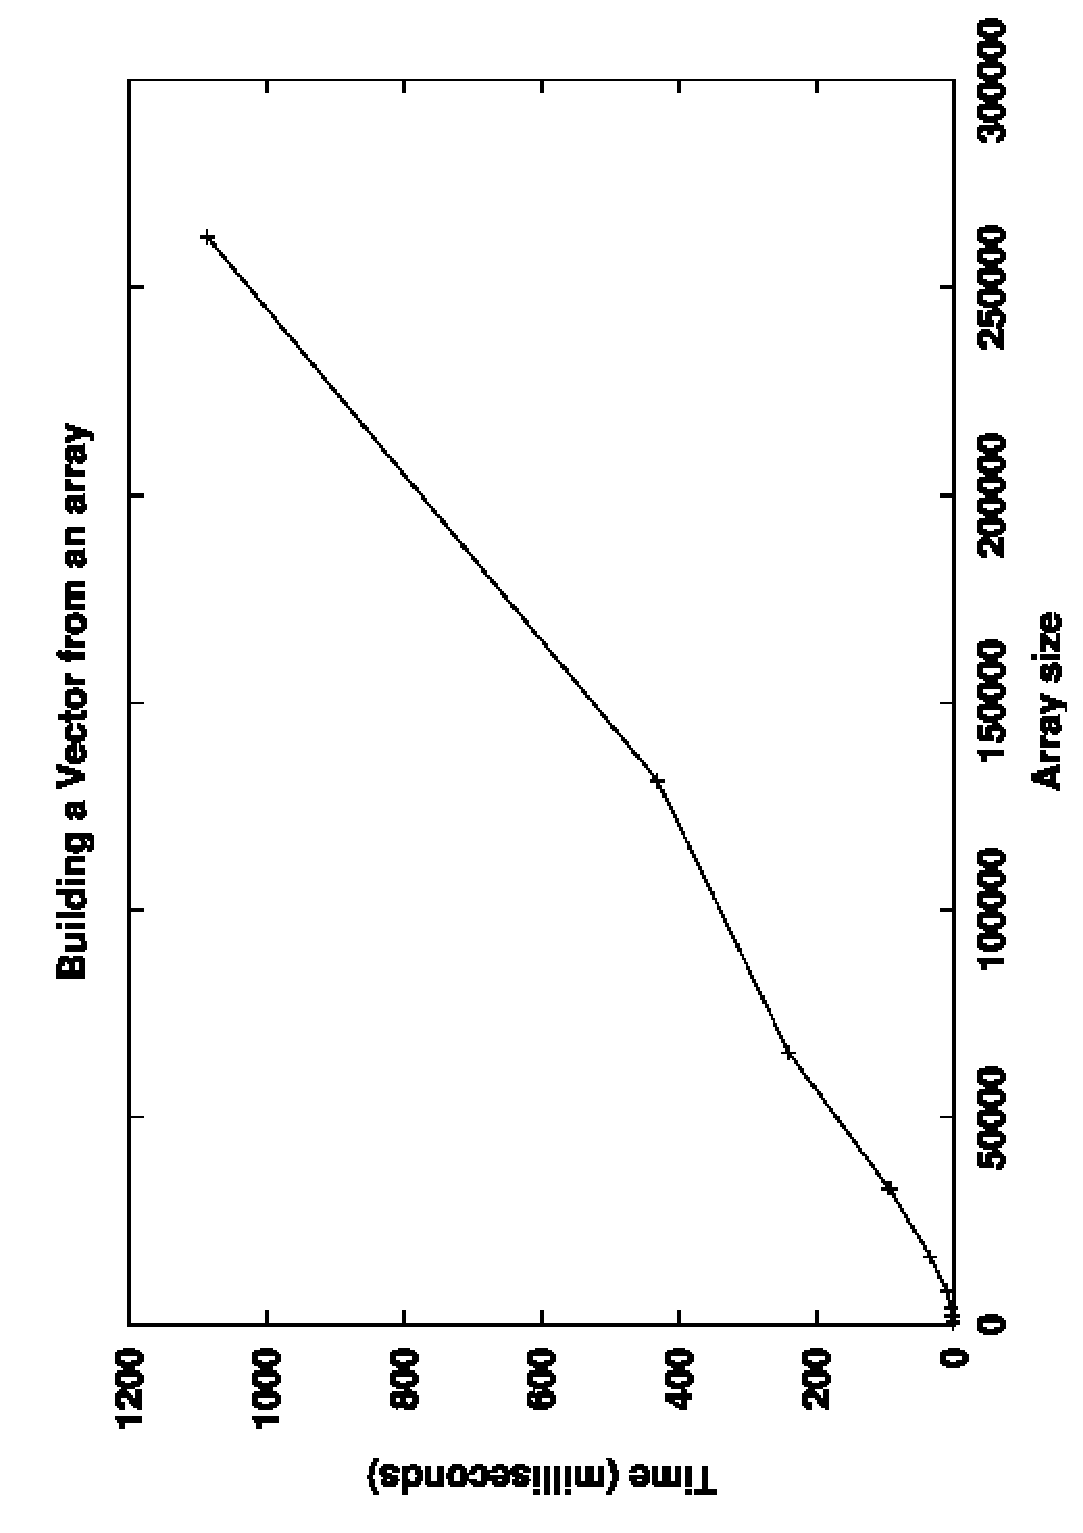
\includegraphics[angle=-90,width=5in]{times.eps}
\end{center}
\caption{Times in milliseconds to build a Vector from various array
sizes. using the code in Figure~\ref{fig:code}}
\label{fig:times}
\end{figure}

Your figures should have a caption that describes exactly what is in
the figure.  A discussion of the figure should be included in your
main text, referring to the figure by number, like so:

The method in Figure~\ref{fig:code} is executed 10 times for each
value of $n$, and the minimum time is taken.  The runs are all done on
a PC with a 700 MHz Intel Pentium III processor, running FreeBSD 4.3
and the Java Development Kit version 1.3.0.  We choose array and
vector sizes starting at $n=512$ and double them until our final size
$n=262,144$.  These bounds, all powers of 2, were chosen because the
512-element case is the first which takes at least one millisecond,
and the 262,144-element is the largest which can execute without
generating an out of memory exception from the Java run-time
environment.  The graph in Figure~\ref{fig:times} shows the actual
execution times for this method.  These times grow linearly with the
size of the array.  This agrees with the expected $O(n)$ behavior.

\section{Writing is Hard}
\label{sec:writing}

As you undoubtedly know, writing is hard.  Turns out, technical
writing is extra hard.  In addition to all of the good things we
should do with spelling, grammar, punctuation, and everything else, we
need to focus on writing for a technical audience.  There is no room
for a wordy writing style.  Our goals are to be concise and precise.
If you can say it in one short sentence instead of a rambling
paragraph, do it!

Here's an example of a before and after.  Before editing:

The experiment was actually set up first.  After we set up the
experiment, we ran the experiment on all of our test cases.  These
test cases are very interesting, as we carefully selected them to be
just that.  Running the experiment allowed us to gather the timings we
present below.  The timings show a trend that looks like a linear
relationship between the input parameter and time taken.  This matches
the theoretical expectation, which is good.

After:

We set up and run our experiment on a set of carefully selected test
cases.  Results, shown below, suggest a linear relationship between
the input parameter and time taken, matching theoretical expectations.

It is perfectly reasonable to write the first paragraph initially.
However, subsequent editing, ideally by multiple people, should lead
to the much more concise and precise second paragraph.

Technical writing is a learned skill, so do not be surprised if your
early versions come under heavy editing and constructive criticism.
That said, even the most experienced technical writers need to make
multiple editing passes.

Here are a few more tips to keep in mind.

\begin{itemize}

\item Define all terms, abbreviations, and acronyms the first time you
  use them.  You should not assume your reader is aware of them, and
  it is annoying, as a reader, to feel the need to stop reading to
  look up a term or acronym.

\item Avoid contractions.

\item Carefully consider the voice to use and be consistent.
  Descriptions of work done is often done using ``we'' even in the
  case of a single author.  Avoid using too much of a storytelling
  approach.

\end{itemize}


\section{Subsections, Math, Tables, Citations}
\label{sec:subsections}

Now back to more of what \LaTeX{} can do and how to present some
common components of a technical paper.  I have subsections here.  I
can label those and refer to them as Sections~\ref{sec:subsection1}
and~\ref{sec:subsection2}.

\subsection{Part 1}
\label{sec:subsection1}

Subsections are fun.  So is math mode: $f(x) = x^4 + a_0 + x^{2k}$ is
nice, but how about $\frac{\alpha}{2} + \log x^y$?  Tip: see the file
\url{isoent-ref.pdf} for 30 pages
of special characters and how to make \LaTeX print them.

\subsection{Part 2}
\label{sec:subsection2}

Did you like the equations in Section~\ref{sec:subsection1}?  How
about a table?

{\singlespace  % since the table looks funny when double-spacing is
	       % left on
\begin{table}[htb]
\begin{center}
\begin{tabular}{|l|l|c|c|l|}
\hline
{\bf Architecture} & {\bf IPC vehicle} & {\bf Procs.} & {\bf
Computers} & {\bf Key}
\\ \hline \hline
IBM SP2 & switch & 2--32 & 2--32 & SP2s \\ \hline
IBM SP2 & Ethernet & 2--32 & 2--32 & SP2e \\ \hline
Sun Ultra 2/2200 & shared memory & 1--2 & 1 & SUNsh \\ \hline
Sun Ultra 2/2200 & local p4 & 1--2 & 1 & SUNlp4 \\ \hline
Sun Ultra 2/2200 & Ethernet p4 & 1--6 & 1--3 & SUNp4(10) \\ \hline
Sun Ultra 2/2200 & fast Ethernet p4 & 1--6 & 1--3 & SUNp4(100) \\ \hline
SGI Onyx II & shared memory & 1--8 & 1 & SGIsh \\ \hline
SGI Onyx II & local p4 & 1--8 & 1 & SGIlp4 \\ \hline
\end{tabular}
\end{center}
\caption{Parallel environments for network performance
comparisons.  Variations in architecture, interprocess communication
vehicles, numbers of processes and computers are examined.}
\label{tab:machines}
\end{table}
}

I made Table~\ref{tab:machines}.  Isn't it nice?  It also has a
caption that describes exactly what the table is supposed to show.
This is an example of how figures and tables can float around.  This
is usually a good thing, and \LaTeX will do something reasonable.
However, it is another reason that captions must describe figures and
tables well, and that the text should refer to them as ``Table X''
rather than ``the following table.''

It is essential that you include all appropriate references.  Maybe
you used something by Barnard and Simon~\cite{barnard94a}.  Or perhaps
you want to say that several papers discuss a point you are making in
more detail~\cite{beall98a,einstein}.  I'll include a few more so you
can see examples of more types of
citations~\cite{gzip,binks99,sagan94a}.  Generally, it is better to
cite a published work rather than a URL.  If you use information from
a web page, try to find books, journal articles, conference
proceedings, or technical reports that contain the same information.
When citing web pages, try to include an accurate title and author.
Tip: open the bibtex file in emacs, and the ``Entry-Types'' menu will
give you a bunch of other templates you can use.

Lists of items are also fun.  Maybe you want bullets:

\begin{itemize}

\item Item 1.

\item Item 2.

  \begin{itemize}
   \item subitem of 2!
   \item another subitem of 2.
  \end{itemize}

\end{itemize}

Maybe you want them numbered:

\begin{enumerate}

\item I bet this gets 1.

\item And this gets 2.

\end{enumerate}

\noindent
Hey!  This paragraph isn't indented.  Sometimes that is what you
want.  And you can do it.

\section{Compiling}
\label{sec:building}

To compile this file into a device independent ({\tt .dvi}) file:

\begin{verbatim}
latex paper.tex
\end{verbatim}

Most of the time, you want PDF:

\begin{verbatim}
pdflatex paper.tex
\end{verbatim}

The procedure above will not include any of your citations.  To get
those, also run
\begin{verbatim}
bibtex paper
\end{verbatim}
after you have run latex once, then rerun the latex command, at least
twice.  Since latex is a one-pass compiler, it relies on information
it stores from previous runs to generate labels and citations and
other information.  If things seem weird, just rerun latex twice and
most of the time, things will be fine.

The included Makefile should do all of this automatically, as long as
you use GNU make ({\tt gmake}).

\section{Conclusions}
\label{sec:conclusions}

Summary, conclusions, discussion of the results, and ideas for future
work should be here.

Again, remember that writing is hard and writing well is very hard.  It
requires a long cycle of writing, reading, editing, rearranging,
rewriting, and so on.  If you are working in a group, have all group
members read and edit each others' sections.  Scientific writing
should be clear and concise.  If find a paragraph that says what can
be said in a sentence, cut it down to one sentence!

% it's nice to acknowledge any person or organization that helped out
% along the way.  The * after \section means this will not be assigned
% a section number
\section*{Acknowledgments}

The authors would like to thank all of our system administrators, past
and present, for installing the tools we needed on our systems and for
keeping those systems working smoothly while we completed this
project.

% Finally, the citations.  These lines tell latex what style to use
% (abbrv means to use first and middle initials instead of full names,
% among other things), and that your bibtex file is called
% references.bib
%
% bibtex alone should be enough to make anyone abandon any wysiwyg
% word processor and use latex for everything!
% 
% we'll also turn off double spacing for the citations
\singlespace
\bibliographystyle{abbrv}
\bibliography{references}

% tell latex we're done.  Anything beyond this line will be ignored.
\end{document}

This doesn't show up, because it came after the \end{document}
